\documentclass[fontset=ubuntu,zihao=-4,a4paper]{ctexart}

%% 目录
\usepackage{titletoc}
\titlecontents{section}[3.8em]
{\songti\zihao{-4}}
{\contentslabel{4em}}{\hspace*{-4em}}
{~\titlerule*[0.8pc]{$.$}~\contentspage}

%% 字体
\setmainfont{Times New Roman}
%\setmonofont{Source Code Pro}
%\setmonofont{Droid Sans Mono}
\setmonofont[Path=font/]{Monaco.ttf}
\newcommand{\zhongsong}{\CJKfontspec[Path=font/]{STZhongSong.ttf}}	%华文中宋
\ctexset{
	section = {
        % format = \centering\bfseries\zihao{-2} \heiti,
		format = \centering\zihao{-2} \heiti,
		name = {第, 章}
	},
	subsection = {
        % format = \bfseries\zihao{3} \heiti
		format = \zihao{3} \heiti
	},
	subsubsection = {
        % format = \bfseries\zihao{4} \heiti
		format = \zihao{4} \heiti
	}
}

%% 交叉引用
\usepackage{hyperref}

%% 代码块
\usepackage{listings}
\usepackage{color}
\definecolor{lightgray}{RGB}{244,247,248}
\definecolor{darkgray}{rgb}{.4,.4,.4}
\definecolor{purple}{rgb}{0.65, 0.12, 0.82}

\lstdefinelanguage{JavaScript}{
  keywords={typeof, new, true, false, catch, function, return, null, catch, switch, var, if, in, while, do, else, case, break},
  keywordstyle=\color{purple}\bfseries,
  ndkeywords={class, export, boolean, throw, implements, import, this},
  ndkeywordstyle=\color{red}\bfseries,
  identifierstyle=\color{black},
  sensitive=false,
  comment=[l]{//},
  morecomment=[s]{/*}{*/},
  commentstyle=\color{darkgray}\ttfamily,
  stringstyle=\color{blue}\ttfamily,
  morestring=[b]',
  morestring=[b]"
}

\lstset{
   language=JavaScript,
   backgroundcolor=\color{lightgray},
   extendedchars=true,
   basicstyle=\footnotesize\ttfamily,
   showstringspaces=false,
   showspaces=false,
   numbers=left,
   numberstyle=\footnotesize,
   numbersep=9pt,
   tabsize=2,
   breaklines=true,
   showtabs=false,
   captionpos=b
}

%% 图形支持宏包
\usepackage{graphicx}               % 嵌入png图像,修改表格的整体大小
\usepackage{booktabs}               % 三线表格中的上中下直线线型设置宏包
\usepackage{tabularx}               % 调整表格宽度,代替tabular

%% 数学公式
% 学位论文版权使用授权书那边的方块可能用到
\usepackage{amsmath}                % AMS LaTeX宏包
\usepackage{amssymb}                % 用来排版漂亮的数学公式
\usepackage{amsbsy}
\usepackage{mathrsfs}               % 英文花体字体

%% 图表按章节编号
\numberwithin{figure}{section}
\numberwithin{table}{section}

%% 设置图标的caption没有冒号
\usepackage{caption}
% \captionsetup[table]{labelsep=space}
\DeclareCaptionLabelSeparator{twospace}{\ ~}
\captionsetup{labelsep=twospace}

%% 页边距调整
\usepackage{setspace}				%设置间距
\usepackage{calc}                   %包含textwidth,textheight
\usepackage{geometry}                
\geometry{top=2.5cm,bottom=2cm,left=2.5cm,right=2cm}

%% 设置间距
\setlength{\lineskip}{20pt}                     %设置行间距
\setlength{\parskip}{0.5\baselineskip - 10pt}   %设置段间距

%% 参考文献上标
\newcommand{\upcite}[1]{\textsuperscript{\textsuperscript{\cite{#1}}}}

%% 标题间距
% \RequirePackage[indentafter]{titlesec}          % \titlespacing*
% \titlespacing*{\section}{0pt}{0.5\baselineskip}{0.5\baselineskip}
% \titlespacing*{\subsection}{0pt}{0.5\baselineskip}{0.5\baselineskip}
% \titlespacing*{\subsubsection}{0pt}{0.5\baselineskip}{0.5\baselineskip}

%% 页眉页脚样式的定义方式
\usepackage{fancyhdr}
\fancyhf{} 
% \setlength{\headsep}{20pt}
% \setlength{\headheight}{0cm}
% \setlength{\textwidth}{\paperwidth - 4.5cm}
% \setlength{\textheight}{\paperheight - 6.08cm - \headsep - \footskip}
% \setlength\topmargin{0.17cm}
\fancyhead[C]{\zihao{5}  \songti 武汉理工大学毕业设计(论文)\\}
\fancyfoot[C]{\zihao{5} \thepage}
\renewcommand{\headrulewidth}{0.65pt} 

%%%%%%%%% 正文区 %%%%%%%%%
\begin{document}
%% 论文引用格式
\bibliographystyle{gbt7714-2005}     
%% 封面和前言
%% 封面
\smallskip
\begin{center}
	
\vspace*{2.2cm}
\zhongsong{\zihao{1} 武汉理工大学毕业设计(论文)} \\
\vspace*{3.3cm}
\heiti{\zihao{2} 基于区块链的考试系统的设计与开发 }\\
\vspace*{5.5cm}

\zhongsong
\begin{tabular}{cc}
	\zihao{-2} 学院(系):&\underline{\makebox[7cm][c]{\zihao{-2}计算机科学与技术学院}} \\ 
	\\
	\zihao{-2}专业班级: & \underline{\makebox[7cm][c]{\zihao{-2}软件zy1701}} \\ 
	\\
	\zihao{-2}学生姓名: & \underline{\makebox[7cm][c]{\zihao{-2}林雨钦}} \\ 
	\\
	\zihao{-2}指导教师: & \underline{\makebox[7cm][c]{\zihao{-2}向广利}} \\ 
	\\
\end{tabular} 
\end{center}
\thispagestyle{empty}
\clearpage
%% 封面
% \smallskip
% \vspace*{1.7cm}
% \begin{center}
% \begin{figure}[!th]
% \centering
% 
\includegraphics[width=0.7\linewidth]{figure/SchoolName}
% \end{figure}

% \vspace*{1.0cm}
% \zhongsong{\zihao{1} 毕业设计(论文)} \\
% \vspace*{4.0cm}
%  \heiti{\zihao{2} 基于区块链的考试系统的设计与开发}\\
% \vspace*{4.0cm}
% \zhongsong
% % \songti
% \begin{tabular}{cc}
%  \zihao{-2} 学院(系):&\underline{\makebox[7cm][c]{\zihao{-2}计算机科学与技术学院}} \\ 
%  \\
%  \zihao{-2}专业班级: & \underline{\makebox[7cm][c]{\zihao{-2}软件zy1701}} \\ 
%  \\
%  \zihao{-2}学生姓名: & \underline{\makebox[7cm][c]{\zihao{-2}林雨钦}} \\ 
%  \\
%  \zihao{-2}指导教师: & \underline{\makebox[7cm][c]{\zihao{-2}向广利}} \\ 
%  \\
% \end{tabular} 
% \end{center}
% \thispagestyle{empty}
% \clearpage

%%%%%%%%% 原创性声明 %%%%%%%%%
\begin{center}
\zihao{-2} \textbf{学位论文原创性声明}
\end{center}

本人郑重声明:所呈交的论文是本人在导师的指导下独立进行研究所取得的研究成果。除了文中特别加以标注引用的内容外,本论文不包括任何其他个人或集体已经发表或撰写的成果作品。本人完全意识到本声明的法律后果由本人承担。 
\begin{flushright}
\zihao{4} 作者签名:\qquad ~~~\\

年\qquad 月\qquad 日
\end{flushright}
\vskip 2cm
\begin{center}
\zihao{-2} \textbf{学位论文版权使用授权书}
\end{center}

本学位论文作者完全了解学校有关保障、使用学位论文的规定,同意学校保留并向有关学位论文管理部门或机构送交论文的复印件和电子版,允许论文被查阅和借阅。本人授权省级优秀学士论文评选机构将本学位论文的全部或部分内容编入有关数据进行检索,可以采用影印、缩印或扫描等复制手段保存和汇编本学位论文。\smallskip

本学位论文属于
\begin{tabular}[t]{l}
1、保密$ \Box$,在~~~年解密后适用本授权书  \\ 
2、不保密$ \Box$  \\ 
\end{tabular} \\
\begin{center}
(请在以上相应方框内打“$\surd”$)
\end{center}
\begin{flushright}
\zihao{4} 作者签名:  \quad\quad\quad\quad 年 \quad  月  \quad  日\\
导师签名:   \quad\quad\quad\quad 年 \quad  月 \quad   日\\
\end{flushright}
\thispagestyle{empty}
\clearpage
\pagestyle{plain}
\pagenumbering{Roman}
\section*{\centering 摘要}
\vskip0.5cm
自区块链技术被确立为我国信息、科技领域的“顶层设计”,区块链作为核心技术的应用也愈发广泛。受新冠疫情的影响,线上教学在全国范围内迅速普及,一个交互好用、功能完备的线上考试系统作为线上教学的配套,十分重要。在2016年国家发布了《国家信息化发展战略纲要》,提倡要加强信息技术领域前沿的基础设施建设。因此,在这样的政策和社会背景下,借区块链技术所提供的数据安全方面的保障能力,提出了一种「基于区块链技术的考试系统」解决方案。项目采用了前后端分离的解耦项目模型,其中前后端都采用了时下流行、成熟、经过企业级项目应用的检验的 SpringBoot 与 Vue。并且,使用新兴的国产区块链底层框架 Fisco Bcos,作为项目中区块链的技术实现。以此,提供一个操作简易、交互友好且数据安全  的线上考试系统,减轻老师工作流程中的负担,提高学校的管理效率。

\textbf{关键词:} 区块链;Fisco Bcos;在线考试系统;SpringBoot;Vue
% \addcontentsline{toc}{section}{摘要}    % 目录中加入

\clearpage  % 分页

\section*{\centering \textbf{Abstract}}
\vskip0.5cm
Since blockchain technology has been established as the "top-level design" in China's information and technology fields, the application of blockchain as a core technology has become more and more widespread. Due to the impact of the new crown epidemic, online teaching is rapidly spreading across the country, and it is important to have an interactive and functional online examination system as a complement to online teaching. In 2016, the country released the "Outline of National Information Development Strategy", advocating the need to strengthen infrastructure construction at the forefront of information technology. Therefore, in such a policy and social context, a solution of "blockchain technology-based examination system" is proposed by taking advantage of the data security aspect guarantee capability provided by blockchain technology. The project adopts the decoupled project model of front-end and back-end, in which SpringBoot and Vue, which are popular, mature and tested in enterprise-level projects, are used for both front-end and back-end, and Fisco Bcos, an emerging domestic blockchain underlying framework, is used as the technical implementation of blockchain in the project. In order to provide an easy-to-use, interactive and data-secure online examination system, to reduce the burden of teachers' workflow and improve the efficiency of school management.

\textbf{Key Words:} Block-chain; Fiscos Bcos; Online Exam-system; SpringBoot; Vue
% \addcontentsline{toc}{section}{Abstract}    % 目录中加入
%% 目录
\pagestyle{empty}
\tableofcontents 
\thispagestyle{empty}
\newpage                            %使得后面页码从1开始

%% 论文正文
\pagestyle{fancy}

% \newpage
% 如你所见,本页为了解决这个第一行文字与页眉分割线重合问题,我们添加了一个空白页。
% \vspace*{\fill}
% \begin{center}   
% 	{\color{red}\fontsize{50} 1此页记得删除}
% \end{center}
% \vspace*{\fill}
% \newpage

\pagenumbering{arabic}                          %后面用阿拉伯数字记页码
\setlength{\lineskip}{20pt}                     %设置行间距
\setlength{\parskip}{0.5\baselineskip - 10pt}   %设置段间距

\section{绪论}
\subsection{背景研究}
2016年7月,中共中央、国务院办公厅印发了《国家信息化发展战略纲要》,规范和指导了未来10年中央对国家信息化的指导思想和战略方针。信息技术的基础水平和相关产业的发展程度,与国家信息化进程密切相关。《国信纲要》提倡,要加强信息技术领域前沿和基础研究,同时应用相应技术,打造协同发展的产业生态。2020年5月两会期间,多位人大代表和政协委员提出了,关于区块链技术在产业中的应用、促进产业发展升级和数字货币监督监管问题,三大方面的想法与提议。由此可知,区块链已然成为了当下乃至今后十年内,我国科技、信息领域发展的“顶层设计”。在这样的发展潮流下,区块链的落地应用和技术推广如雨后春笋:国家邮政局鼓励以区块链为主要应用核心的新一代技术升级;银保监会为提高数据安全性,在交易环节应用区块链技术;教育部也在《全国大中小学教材建设规划(2019-2022年)》的记者问答中表示,下一步将围绕区块链等新技术领域重点建设,集中力量编写、打造新经典教材。

2020年初的疫情导致近乎所有学生都参与到了线上教学,由此影响,在线课堂、在线考试受到了极大的推广。腾讯会议、钉钉、腾讯课堂等线上视频会议的产品快速迭代之中逐渐成熟。与之相应,也诞生了许多在线考试的相关解决方案,例如超星学习通、中国大学慕课、智慧树。线上考试的方式与传统的线下纸质化考试相比,有如下的优劣之处:

\begin{itemize}
    \item 能够代替教师的部分工作,一定程度上地方便学校、教育机构对考试的安排管理,提高了工作效率;
    \item 有效地缩短考试前期安排的组织周期,减轻了相关通知传递过程中的人力损耗;
    \item 线上交卷、评卷缩短了学生得到考试反馈结果的时间周期;
    \item 在相关硬件设施条件满足的前提下,进一步地保证了考试过程中的公平公正;
    \item 存在线上系统都无法避免的网络攻击风险;
    \item 数据集中化存储管理,有潜在的被篡改等安全问题;
\end{itemize}

如上的在线考试解决方案通常使用了移动端 C/S 结构,桌面端 B/S 结构。如此的客户端-服务端解构模式,实现了在不同的用户前端实现下,用户数据的共通。在这样的项目架构模型中,数据的安全性、可靠性、可信度便显得尤为关键。结合这两个方面,提出本项目「基于区块链技术的线上考试系统」。线上考试系统的方式合理利用了当今时代互联网的便捷性与普及程度。采用国家大力支持推广的区块链技术,可以有效地保证数据存储管理的安全性。

区块链技术最早由中本聪于《比特币:一种点对点的电子现金系统》\textsuperscript{\cite{ref0}}一文中提出,是一种类似于分布式的账本的数据存储与管理技术。在共识机制、工作量证明(PoW)等方式保障下,区块链技术具有:不可篡改、可追溯源、去中心化等特性与优点。这些特点正好与线上考试系统的数据安全方面的问题十分契合:防篡改、可溯源保证了考试数据的安全;去中心化的特性发挥了数据分布式存储的优势,降低了集中化数据存储方式存在的安全风险,减轻了系统服务器压力,加强了数据可用性、系统可用性。将区块链技术应用至系统中,会是诸如线上考试系统此类的数据安全敏感系统今后的更新趋势,也呼应了国家对于区块链技术重视与号召。


\subsection{需求分析}
\subsubsection{目标用户群体}
\begin{itemize}
    \item 学校、教育机构:有固定时间周期性的测试或考试需要,使用线上考试系统可以覆盖一些简单的定期多次小测验;
    \item 学生:无纸化的线上考试系统使得考试结果反馈更加快速;
\end{itemize}

\subsubsection{用户主要目的}
需要一款线上考试系统的解决方案,能方便快捷的满足学校、教育机构平时周期性的测试的需要。教师能够简单的操作就能配置题目、题库、发布试卷,通过预先设定的参考答案,能够自动评卷登分,将考试结果与相关题目解析快速反馈给参与考试的学生。

\subsubsection{功能性需求}
\begin{figure}[htb!]
    \centering
    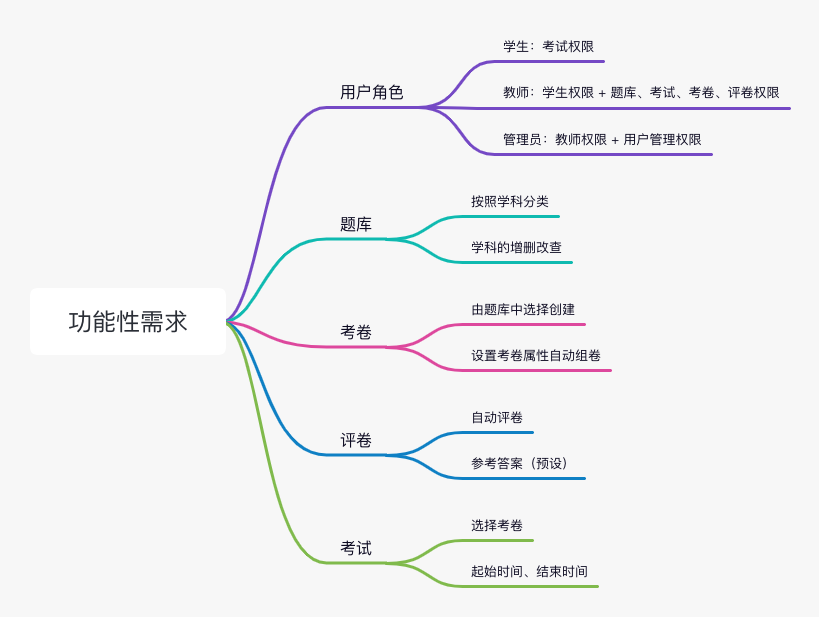
\includegraphics[width=0.8\linewidth]{_images/功能性需求.png}
    \caption{功能性需求}
    \label{功能性需求}
\end{figure}
\paragraph{用户角色分类} 系统的参与者主要分为三类:学生、教师、管理员,学生与教师对应实际业务场景中的角色,管理员是因系统的操作与非业务的操作而存在。
\paragraph{题库功能} 题目作为考卷的基本单位,考卷就是多个题目的组成。项目需要题目的基本管理功能。题目按题型又将分为:单选题、多选题、判断题、填空题等。题目按照学科分类,因此又需要题库功能对不同的学科题目进行管理。
\paragraph{考卷功能} 考卷是考试进行的必要组成部分,考卷需要由教师手动从题库中选择,或是通过设定一定的规则从设定好的题库中抽取自动组卷。考卷也需要基本的增删改查功能。
\paragraph{考试功能} 考试通过选择已创建的考卷而开启,学生可以进入已创建的考试进行线上考试。考试也需要设置起始时间和结束时间属性。
\paragraph{评卷功能} 题目设置的时候提供对应的正确答案选项,使得在作答结束后能够通过正确答案与学生的作答情况自动评卷计分,并提供预先设置的参考题解给学生。
\paragraph{用户管理} 管理员才被允许对系统中的用户进行新增、删除、修改信息、查看。用户也可以对自己的基本信息做修改,例如修改密码、头像、昵称。
\paragraph{权限分类} 根据以上的用户角色分类和功能模块,需要将具体的功能模块访问限制与用户角色对应。学生只允许参与考试和查看自己考试的情况;老师具有学生的所有权限用于考卷的试测,此外需要考卷功能模块、题库功能模块、评卷功能模块的权限;管理员具有所有的功能模块权限,即老师的权限加上用户管理功能模块的权限。

\subsubsection{非功能性需求}
\begin{itemize}
    \item 界面美观,布局简洁大方;
    \item 用户交互操作友好。用户意外的错误操作,或是发生运行时错误,应有合理的信息提示;
    \item 系统使用需要有清晰、完善的文档说明,项目代码注释完善、易读;
    \item 项目需要具有足够的测试性,以保证系统性能可用于实际环境;
    \item 项目结构设计良好、易于维护,并留存有一定后期功能拓展的空间;
    \item 用户操作具有完备的鉴权流程,防止非法操作;
    \item 前端布局弹性,根据不同的分辨率响应式渲染展示;
\end{itemize}


\subsection{进度安排}
\paragraph{2021/1/8 - 2021/2/28} 确定选题,查阅文献,外文翻译和撰写开题报告。这期间主要通过导师提供的相关材料,以及自己查阅相关的文献,熟悉项目题目的研究背景、应用领域、技术生态。在完成了文献查阅和外文文献翻译后,根据自己的这阶段对项目选题的方方面面的理解,撰写开题报告;
\paragraph{2021/3/1 - 2021/3/20} 完成系统核心功能设计,主要包括数据库表设计,对项目中实体的抽象;使用 Vue 及其相关技术栈实现最小 Demo,主要目的是通过实际开发实践巩固所学的前端技术部分的理论知识;熟悉 SpringBoot、Fisco Bcos 等后端部分的技术文档,对业务对象、功能模块的设计实现有一定思考和初步设想,能做到胸有成竹;
\paragraph{2021/3/21 - 2021/4/20} 参考网上成熟的系统界面原型设计,对前端部分的布局和组件抽象有大概的构想;编写项目的核心功能模块的代码,包括前端页面展示部分和后端数据处理部分;
\paragraph{2021/4/21 - 2021/5/11} 尝试与实践区块链的结点部署,并修改项目后端核心实体对象的数据处理,增加区块链接入层,实现安全敏感的重要数据上链;
\paragraph{2021/5/12 - 2021/5/18} 熟悉相关的测试技术,对项目进行单元测试、压力测试等各方面的测试,并记录数据;
\paragraph{2021/5/19 - 2021/5/31} 撰写及修改毕业论文;
\paragraph{2021/6/1 - 2021/6/5} 准备答辩。

\subsection{论文结构安排}
\paragraph{第一章}绪论介绍了在当下的社会政策与技术潮流中,项目的研究和应用意义。以及分析了项目面向的用户群体,用户需求。

\paragraph{第二章}简要介绍了项目所使用的相关技术栈,简要概述了技术选型的思考过程:选用的技术的稳定程度与社区生态;与相似技术及其技术栈对比之中的优劣;与项目开发的适用性。

\paragraph{第三章}介绍了系统的整体设计模型、分层的构思过程,项目系统具体的分工模块,模块间的相互协作。

\paragraph{第四章}重点着眼于项目系统的几个核心模块的代码实现思路,和模块的代码开发中所遇到的难点、个人的思考与解决方式。

\paragraph{第五章}展示了使用相关的测试技术对项目应用时各方面的测试结果与结论。

\paragraph{第六章}总述个人对于项目仍存在的不足之处,和潜在的改进空间。
\section{需求分析}
\subsection{目标用户群体}
\begin{itemize}
    \item 学校、教育机构:有固定时间周期性的测试或考试需要,使用线上考试系统可以覆盖一些简单的定期多次小测验;
    \item 学生:无纸化的线上考试系统使得考试结果反馈更加快速;
\end{itemize}

\subsection{用户主要目的}
需要一款线上考试系统的解决方案,能方便快捷的满足学校、教育机构平时周期性的测试的需要。教师能够简单的操作就能配置题目、题库、发布试卷,通过预先设定的参考答案,能够自动评卷登分,将考试结果与相关题目解析快速反馈给参与考试的学生。

\subsection{功能性需求}
\begin{figure}[htb!]
    \centering
    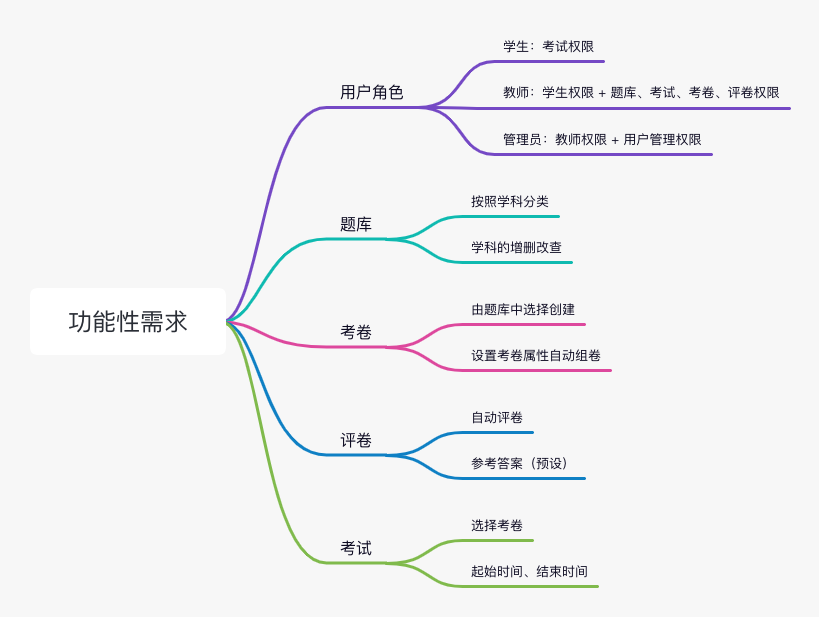
\includegraphics[width=0.8\linewidth]{_images/功能性需求.png}
    \caption{功能性需求}
    \label{功能性需求}
\end{figure}
\paragraph{用户角色分类} 系统的参与者主要分为三类:学生、教师、管理员,学生与教师对应实际业务场景中的角色,管理员是因系统的操作与非业务的操作而存在。\upcite{ref6}
\paragraph{题库功能} 题目作为考卷的基本单位,考卷就是多个题目的组成。项目需要题目的基本管理功能。题目按题型又将分为:单选题、多选题、判断题等。题目按照学科分类,因此又需要题库功能对不同的学科题目进行管理。
\paragraph{考卷功能} 考卷是考试进行的必要组成部分,考卷需要由教师手动从题库中选择,或是通过设定一定的规则从设定好的题库中抽取自动组卷。考卷也需要基本的增删改查功能。
\paragraph{考试功能} 考试通过选择已创建的考卷而开启,学生可以进入已创建的考试进行线上考试。考试也需要设置起始时间和结束时间属性。
\paragraph{评卷功能} 题目设置的时候提供对应的正确答案选项,使得在作答结束后能够通过正确答案与学生的作答情况自动评卷计分,并提供预先设置的参考题解给学生。
\paragraph{用户管理} 管理员才被允许对系统中的用户进行新增、删除、修改信息、查看。用户也可以对自己的基本信息做修改,例如修改密码、头像、昵称。
\paragraph{权限分类} 根据以上的用户角色分类和功能模块,需要将具体的功能模块访问限制与用户角色对应。学生只允许参与考试和查看自己考试的情况;老师具有学生的所有权限用于考卷的试测,此外需要考卷功能模块、题库功能模块、评卷功能模块的权限;管理员具有所有的功能模块权限,即老师的权限加上用户管理功能模块的权限。\upcite{ref3}

\subsection{非功能性需求}
\begin{itemize}
    \item 界面美观,布局简洁大方;
    \item 用户交互操作友好。用户意外的错误操作,或是发生运行时错误,应有合理的信息提示;
    \item 系统使用需要有清晰、完善的文档说明,项目代码注释完善、易读;
    \item 项目需要具有足够的测试性,以保证系统性能可用于实际环境;
    \item 项目结构设计良好、易于维护,并留存有一定后期功能拓展的空间;
    \item 用户操作具有完备的鉴权流程,防止非法操作;
    \item 前端布局弹性,根据不同的分辨率响应式渲染展示;
\end{itemize}

\subsection{章节小结}
本章从目标群体、用户目的、功能性和非功能性需求四个方面对项目的实际业务场景,以及用户的真实需求进行了全面分析和深入探究。

其中主要确定了本项目的核心用户为学校(或教育机构)、教师、学生。进而,围绕着这几个核心用户群体的用户表层需求,去进行深挖、探究其本质的用户需求。从而得出本章节中表述的「功能性需求」部分的总结归纳。除此以外,还基于用户的交互体验和友好性,结合时下主流系统的标准,归纳出项目的非功能性方面的需求。如上的分析都为了项目的前期进展做准备,进而更好的在之后的项目推进中进行系统的设计与开发。
\section{系统设计}
\subsection{总体架构模型设计}
\subsubsection{前端架构模型}
\begin{figure}[htb]
    \centering
    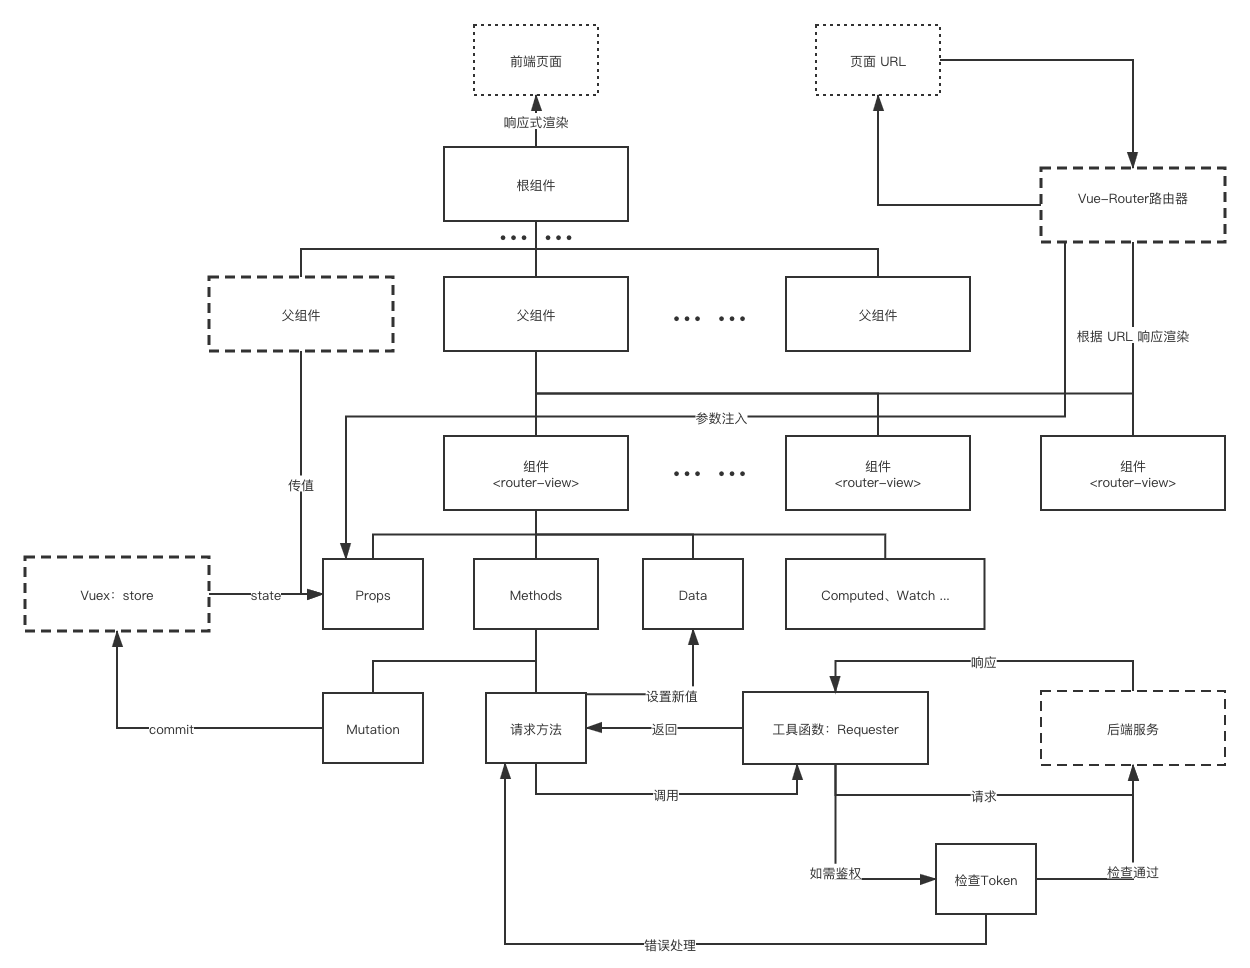
\includegraphics[width=\linewidth]{_images/前端模型.png}
    \caption{前端架构模型}
\end{figure}
Vue 的技术基础是将根节点组件挂载在页面的一个 DOM 元素上,而根节点组件由可由多个组件组成,如此向下细分成子组件。组件系统是 Vue 的另一个重要概念,因为它是一种抽象,允许我们使用小型、独立和通常可复用的组件构建大型应用。\upcite{refAdd19}

组件的数据来源可以划分为:Props、Data、Computed。父子组件之间的数据通信通过 Props,而 Vue 的设计理念中,数据是自上而下单向流动。

面对需要多组件之间共享公共的数据的场景,需要引入 Vuex 的 store。store 将托管的公有数据 state,通过预先在根节点的注册,注入到需要的组件的 Props 中。如有需要对 store 中的数据进行修改,可以将 store 的 mutation 注入到组件的 Methods 中,通过提交(commit)mutation 实现对 store 中的 state 修改。

组件的 Data 也可能来自于用户的交互产生,又或是向后端服务请求的数据。组件中的请求方法,通过调用工具函数 Requester 向后端服务发起请求,其中如有必要应进行 Token 用户令牌的检查。响应得到的数据将返回给请求方法,进而给组件的 Data 赋予新值。

组件的渲染可能受控于父组件的逻辑,也可能受路由器的控制。在父组件中注册成为 <router-view> 的子组件,就通过 Vue-Router 的路由器,根据页面的 URL 动态响应渲染。其中也可以通过页面的 URL 动态路由匹配,向组件的 Props 注入匹配到的参数。


\subsubsection{后端架构模型}
\begin{figure}[htb]
    \centering
    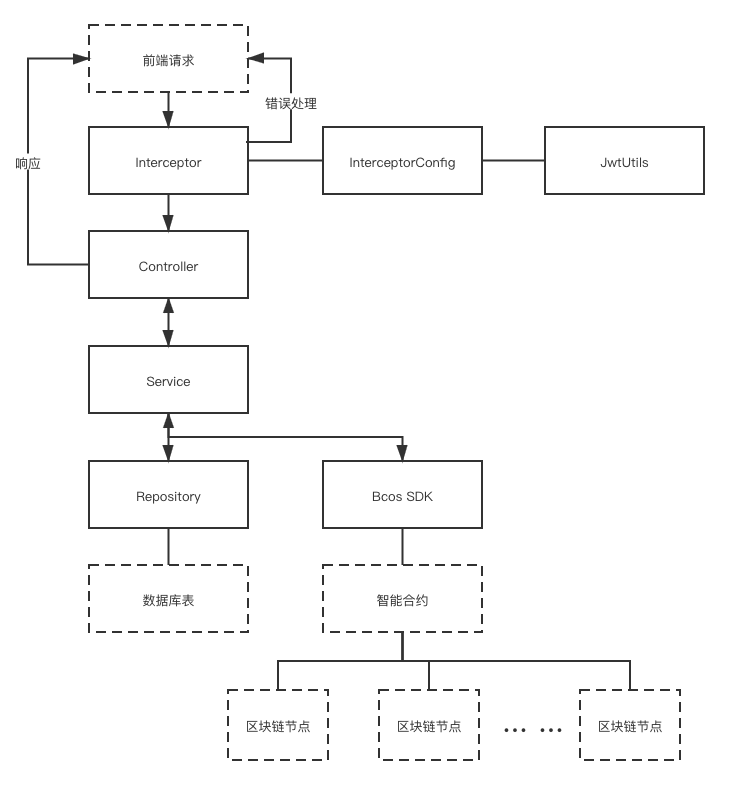
\includegraphics[width=0.85\linewidth]{_images/后端模型.png}
    \caption{后端架构模型}
\end{figure}
前端请求进入后端服务首先会被拦截器 Interceptor 所截获。通过 InterceptorConfig 配置需要拦截的 api 的 url 规则,并加入对应的 Interceptor。项目中的 JWT 鉴权流程便放在拦截器这一层运行。

请求根据具体 api 的 URL,进入不同的 controller,controller 根据业务调用对应的 Service 中的方法。由于使用了 SpringData JPA,数据库中的表与 Repository 对应且关联,因而 Service 中对 DAO 的操作则需要依赖于 Repository。

针对敏感数据需要上链的 Service,通过 Fisco Bcos 提供的 SDK,接入预先编译成 Java 文件的智能合约。而智能合约由通过密钥对的形式连接至区块链节点组成的网络。

\subsection{功能模块划分}
\begin{figure}[htb]
    \centering
    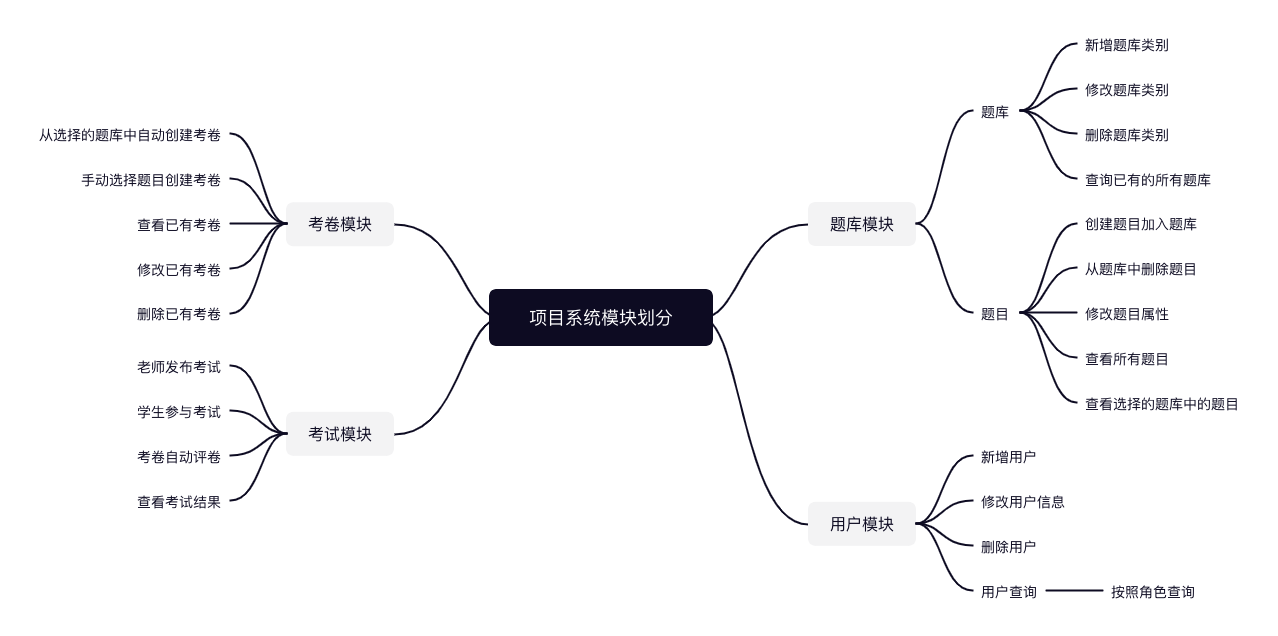
\includegraphics[width=\linewidth]{_images/功能模块划分.png}
    \caption{功能模块划分}
\end{figure}
项目系统根据功能划分成几个功能模块:题库模块、用户模块、考卷模块、考试模块。

按照权限分类用户角色,其对应的功能模块为:\upcite{ref4,refAdd8}
\begin{itemize}
    \item 学生:考试模块
    \item 老师:题库模块、考试模块、考卷模块
    \item 管理员:题库模块、考试模块、考卷模块、用户模块
\end{itemize}

\subsection{Http 请求响应设计}
\subsubsection{前端请求}
\noindent\textit{front/Requester.js/post函数}
\begin{lstlisting}
function post(url, params = {}, needToken = true) {
    const {token} = TokenManager.getToken()
    ... ...
    Logger.log('request', {url, params})
    return axios({
        method: 'post',
        url: url,
        responseType: 'json',
        data: params,
        headers
    }).then(response => {
        const {data, status, statusText} = response
        Logger.log('response', data)
        return data
    }).catch(reason => {
        const {status, statusText} = reason.response
        Logger.error('response', status, statusText, reason.response)
        throw reason.response
    })
}
\end{lstlisting}
前端的请求发起主要依赖于基于 xhr 实现的第三方库 axios。axios 由于请求的异步延时特性,所以使用了 Promise 进行了封装。

前端对后端的请求过程中,请求的 url 前缀部分都是相同的。此外,对于常用的 POST、GET 方法,请求头部分也有相似的部分,例如,POST 请求统一使用「application/json」的 content-type,并将具体的请求数据 json 序列化后,通过 axios 的 data 字段写入请求体中。因而,可以对 axios 再做一层定制,封装成项目的工具函数集合 Requester 中 post、get。

在业务流程中,使用 Requester,仅仅需要根据请求的方法,调用对应的 post、get,传入对应的 api 的 url、请求参数 params,和是否需要 token 验证的标志位 needToken。而无需关心其中具体的请求配置,以及响应的错误处理。获取响应以后再通过一层 Promise 解构其中真正需要的响应数据,使得在业务层面对于请求-响应中的细节是透明无感知的,从实际意义上的减轻了业务开发过程中的心智负担。并可以在工具函数 Requester 中加入日志输出,以便在线上部署后,通过日志迅速定位错误信息。

\subsubsection{后端响应}
\noindent\textit{back/ResultVO.java}
\begin{lstlisting}[language=Java] 
@Data
@JsonInclude(JsonInclude.Include.NON_NULL) 
public class ResultVO<T> {

    public ResultVO(Integer code, String msg, T data) {
        this.code = code;
        this.msg = msg;
        this.data = data;
    }

    public ResultVO() {}

    private Integer code;

    private String msg = "";

    private T data;
}
\end{lstlisting}

\noindent\textit{back/ExamController.java/getExamRecordList函数}
\begin{lstlisting}[language=Java]
@GetMapping("/record/list")
@ApiOperation("获取当前用户的考试记录")
ResultVO<List<ExamRecordVo>> getExamRecordList(HttpServletRequest request) {
    ResultVO<List<ExamRecordVo>> resultVO;
    try {
        // 拦截器里设置上的用户id
        String userId = (String) request.getAttribute("user_id");
        // 下面根据用户账号拿到他(她所有的考试信息),注意要用VO封装下
        List<ExamRecordVo> examRecordVoList = examService.getExamRecordList(userId);
        resultVO = new ResultVO<>(0, "获取考试记录成功", examRecordVoList);
    } catch (Exception e) {
        e.printStackTrace();
        resultVO = new ResultVO<>(-1, "获取考试记录失败", null);
    }
    return resultVO;
}
\end{lstlisting}

后端的响应部分更多的是借助 SpringBoot 中 \lstinline!starter-web! 启动器所提供的相关框架能力。针对响应体的自定义封装,主要是使用了 ResultVO 这一值对象(Value Object)。其中定义了针对业务而言的状态码 code,即业务操作成功为 0,业务操作失败则为非 0。随之附带 msg 作为扩展的信息说明字段。并且 \lstinline!ResultVO! 通过泛型 \lstinline!<T>! 注入具体响应时的数据类型。例如,\lstinline!getExamRecordList! 函数中展示的,针对当前业务操作需要的是 \lstinline!List<ExamRecordVo>! 的数据类型,因而,在 try-catch 前初始化的响应结果 \lstinline!resultVO! 就是 \lstinline!ResultVO<List<ExamRecordVo>>!。

\subsection{鉴权设计}
针对前后端分离的项目结构,鉴权设计主要是借助 JWT(JavaScript Web Token)这一通用的解决方案完成。
\subsubsection{前端鉴权}
\noindent\textit{front/TokenManager.js}
\begin{lstlisting}[language=JavaScript]
// 设置 Token
function setToken({token, userInfo}, remember = false) {
    if (remember) {
        // 写入 localStorage
        localStorage.setItem(...)
    }
    // 在 store 中设置值
    store.commit(...)
    ... ...
}

// 获取 Token
function getToken() {
    let token, userInfo
    if (store.getters.getToken) {
        token = store.getters.getToken
    }
    if (store.state.auth.userInfo) {
        userInfo = store.state.auth.userInfo
    }
    if (!token && localStorage.getItem(tokenKey)) {
        token = localStorage.getItem(tokenKey)
        userInfo = JSON.parse(localStorage.getItem(userInfoKey))
        // 在 store 中设置值
        store.commit(...)
        ... ...
    }
    return {
        token, userInfo
    }
}

// 移除 Token
function removeToken() {
    ... ...
}
\end{lstlisting}
前端部分对于 Token,以及可以与 Token 视作相关联的敏感用户信息 UserInfo,都使用相同的存储管理思路。

针对登录时勾选了“记住登录状态”的情况,将 Token 以及 UserInfo 写入浏览器提供的 localStorage 中。localStorage 是浏览器提供的一种缓存能力,写入 localStorage 中的键值对,可以持久化存储,使得在浏览器退出后也不会丢失。

针对普通的登录情况,则将这些重要数据写入 Vuex 提供的 store 中,方便各组件获取和修改。

如果重新打开浏览器进入页面,且有勾选“记住登录状态”的情况,store 中已有的 Token 是因为进程退出而丢失的,然而 localStorage 中可能还存有未过期的 Token。因而,在 TokenManager 的 getToken 函数中,需要首先检查 store 中是否有保存 Token,如果没有则再在 localStorage 中读取。如果 localStorage 中读取成功,则说明用户是有勾选了“记住登录状态”,则需要将 Token 作为函数返回值之前,将读取到的 Token 存储到 store 中。

Token 存储的情况有多种,但是移除的时候无需关心是否存在,只需要一并清空 store 和 localStorage 中可能存在的键值对即可。

\noindent\textit{front/Requester.js/post函数}
\begin{lstlisting}[language=JavaScript]
function post(url, params = {}, needToken = true) {
    const {token} = TokenManager.getToken()
    if (needToken && !token) {
        Logger.error('not found token')
        return Promise.reject({
            code: 1401,  // 浏览器的401
            msg: 'not found token'
        })
    }
    const headers = {}
    if (needToken) {
        headers['Access-Token'] = `bearer ${token}`
    }
    ... ...
}
\end{lstlisting}

在 Requester 工具函数中,请求如果设置了 needToken 的标志位,则使用 TokenManager 的 getToken 函数中读取可能存在的 Token。如此设计,在请求的代码编写中,将两个模块解耦,仅仅通过函数调用相互关联,符合“高内聚,低耦合”的设计原则。

如果需要 Token 而 getToken 无法返回有效 Token 时,则需要进行错误的处理。遵照 axios 的 Promise 风格 api,错误处理也使用相似的 Promise.reject。其中自定义状态码设置为“1401”,意图借 HTTP 状态码的 401 相同的含义,再前加上 1,以示区别。

getToken 成功返回 Token 后,则通过请求头中的 Access-Token 字段,在请求中携带上 Token。

\noindent\textit{front/Requester.js/handleRequestError函数}
\begin{lstlisting}[language=JavaScript]
function handleRequestError(error) {
    if (
        (
            error && typeof (error) === 'object' &&
            error.code > 1400 && error.code < 1500
        ) || error.status === 401
    ) {
        TokenManager.removeToken()
    }
    Logger.error(error)
}
\end{lstlisting}

对于如上的需要 Token,而又没有 Token 的特殊处理情况,则通过 handleRequestError 对于前面定义的特殊状态码“1401”做处理动作,在当前的项目中,仅仅只是调用了 removeToken。但是,将这个针对 Token 的错误处理环节的独立抽离,也是意图方便以后可能会加入的新的错误处理逻辑,使得项目代码留存有一定的扩展空间。

\subsubsection{后端鉴权}
\noindent\textit{back/LoginInterceptor.java/preHandle函数}
\begin{lstlisting}[language=Java]
@Override
public boolean preHandle(... ...) throws Exception {
    ... ...
    // 注意要和前端适配Access-Token属性,前端会在登陆后的每个接口请求头加Access-Token属性
    String token = request.getHeader("Access-Token");
    ... ...
    if (token != null) {
        // 请求中是携带参数的
        Claims claims = JwtUtils.checkJWT(token);
        if (claims == null) {
            // 返回null说明用户篡改了token,导致校验失败
            sendJsonMessage(response, JsonData.buildError("token无效,请重新登录"));
            return false;
        }
        ... ...
        return true;
    }
    ... ...
    return false;
}
\end{lstlisting}
后端的鉴权与前端部分相对应,而后端的请求鉴权主要是通过 SpringBoot 提供的拦截器 \lstinline!Interceptor! 框架能力完成。\upcite{refAdd9}拦截器通过配置对应的拦截规则,调用对应的拦截器,可以实现需要鉴权的请求在进入实际的业务代码 \lstinline!Controller! 层之前,在拦截器中进行鉴权。将其这部分鉴权逻辑单独通过拦截器实现,目的是为了同业务代码独立开,互相不影响。如此的设计,也是遵从了“低耦合”的原则思想。
\begin{lstlisting}[language=Java]
public class JwtUtils {
    // 构建 token 的主题
    private static final String SUBJECT = ... ...;
    // 过期时间为1天
    private static final long EXPIRE = 1000 * 60 * 60 * 24;

    private static final String APP_SECRET = ... ...;

    public static String genJsonWebToken(User user) {
        ... ...
        return Jwts.builder().setSubject(SUBJECT)
                // 下面3行设置 token 中间字段,携带用户的信息
                ... ...
                // 设置过期时间
                ... ...
                // 生成的结果字符串太长,这里压缩下
                .compact();
    }

    /* 校验 token */
    public static Claims checkJWT(String token) {
        ... ...
    }
}
\end{lstlisting}

将 jsonwebtoken 提供的 api 能力针对项目的业务情况再进行一次封装,成为 \lstinline!JwtUtils! 工具。对外仅提供了对 Token 的创建、校验能力。

\subsection{数据库结构设计}
\subsubsection{数据库概念设计}
\begin{figure}[htb]
    \centering
    \includegraphics[width=\linewidth]{_images/ER图.png}
    \caption{数据库ER图}
\end{figure}

\subsubsection{数据库逻辑设计}
\begin{lstlisting}
users(
    userId, username, password, roleId, avatar,
    nickname, description, createTime, updateTime
)
exam_paper( examPaperId, name, avatar, questionIds, score, creatorId )
exam( id, name, avatar, startDate, endDate, timeLimit, creatorId )
question_bank( id, name, questionIds, creatorId, ... )
question( id, name, description, optionIds, ... )
\end{lstlisting}
\subsubsection{数据表字段说明}
\paragraph{users}
\begin{itemize}
    \item userId 为表的主键,用于唯一标识一个用户;
    \item username 为用户的登录时所用名称,与 userId 一样不可重复;
    \item avatar 存储用户头像;
    \item roleId 存储用户对应的权限角色的枚举值;
    \item nickname 存放用户的昵称,可重复,仅用于展示;
    \item password 为用户登录时所使用的密码;
\end{itemize}
\paragraph{exam\_paper}
\begin{itemize}
    \item examPaperId 为表的主键,用于唯一标识一张考卷;
    \item name 存放考卷的名称;
    \item avatar 存放考卷的封面,可为空;
    \item questionIds 存放考卷拥有的题目的 id 集合;
    \item score 表示考卷的总分值;
    \item creatorId 存放创建考卷的用户的 id(外键);
\end{itemize}
\paragraph{exam}
\begin{itemize}
    \item id 为表的主键,用于唯一标识一场考试;
    \item name 表示考试的名称;
    \item startDate、endDate 表示考试的有效日期范围;
    \item timeLimit 表示考试的答题时间;
    \item creatorId 存放创建考试的用户的 id(外键);
\end{itemize}

\subsection{章节小结}
本章主要针对项目的实际开发,基于前一章节需求分析的相应要求,进行了模块层面的构思和设计。

首先从项目的架构模型进行入手,由于采用的是前后端分离的B/S模型,所以总体的架构模型也分为前后端两个方面去进行设计。其中区块链存储数据的接入层也被归整于后端的模型设计中。

针对需求分析章节中的功能性模块分析,抽象整合出了相应的项目的核心模块划分。之后的项目代码开发也将以此作为开发设计的基础。

此外还着重对项目中使用的核心技术实现做了一定的设计。诸如前后端交互中,请求响应通信交互过程中的逻辑设计。以及用户对项目功能使用的权限划分中尤为重要的鉴权过程的逻辑设计,和对实际项目使用的过程中,鉴权部分可能出现的问题,针对性地进行了代码层面的覆盖。

最后是对项目的实际业务流程中的实体(Entity)进行了抽象,分析了相互之间的关系(Relation),和其必要的属性。主要通过E-R图和数据库表结构设计的方式展现。
\section{系统实现}
\subsection{题库模块}
\begin{figure}[hb]
    \centering
    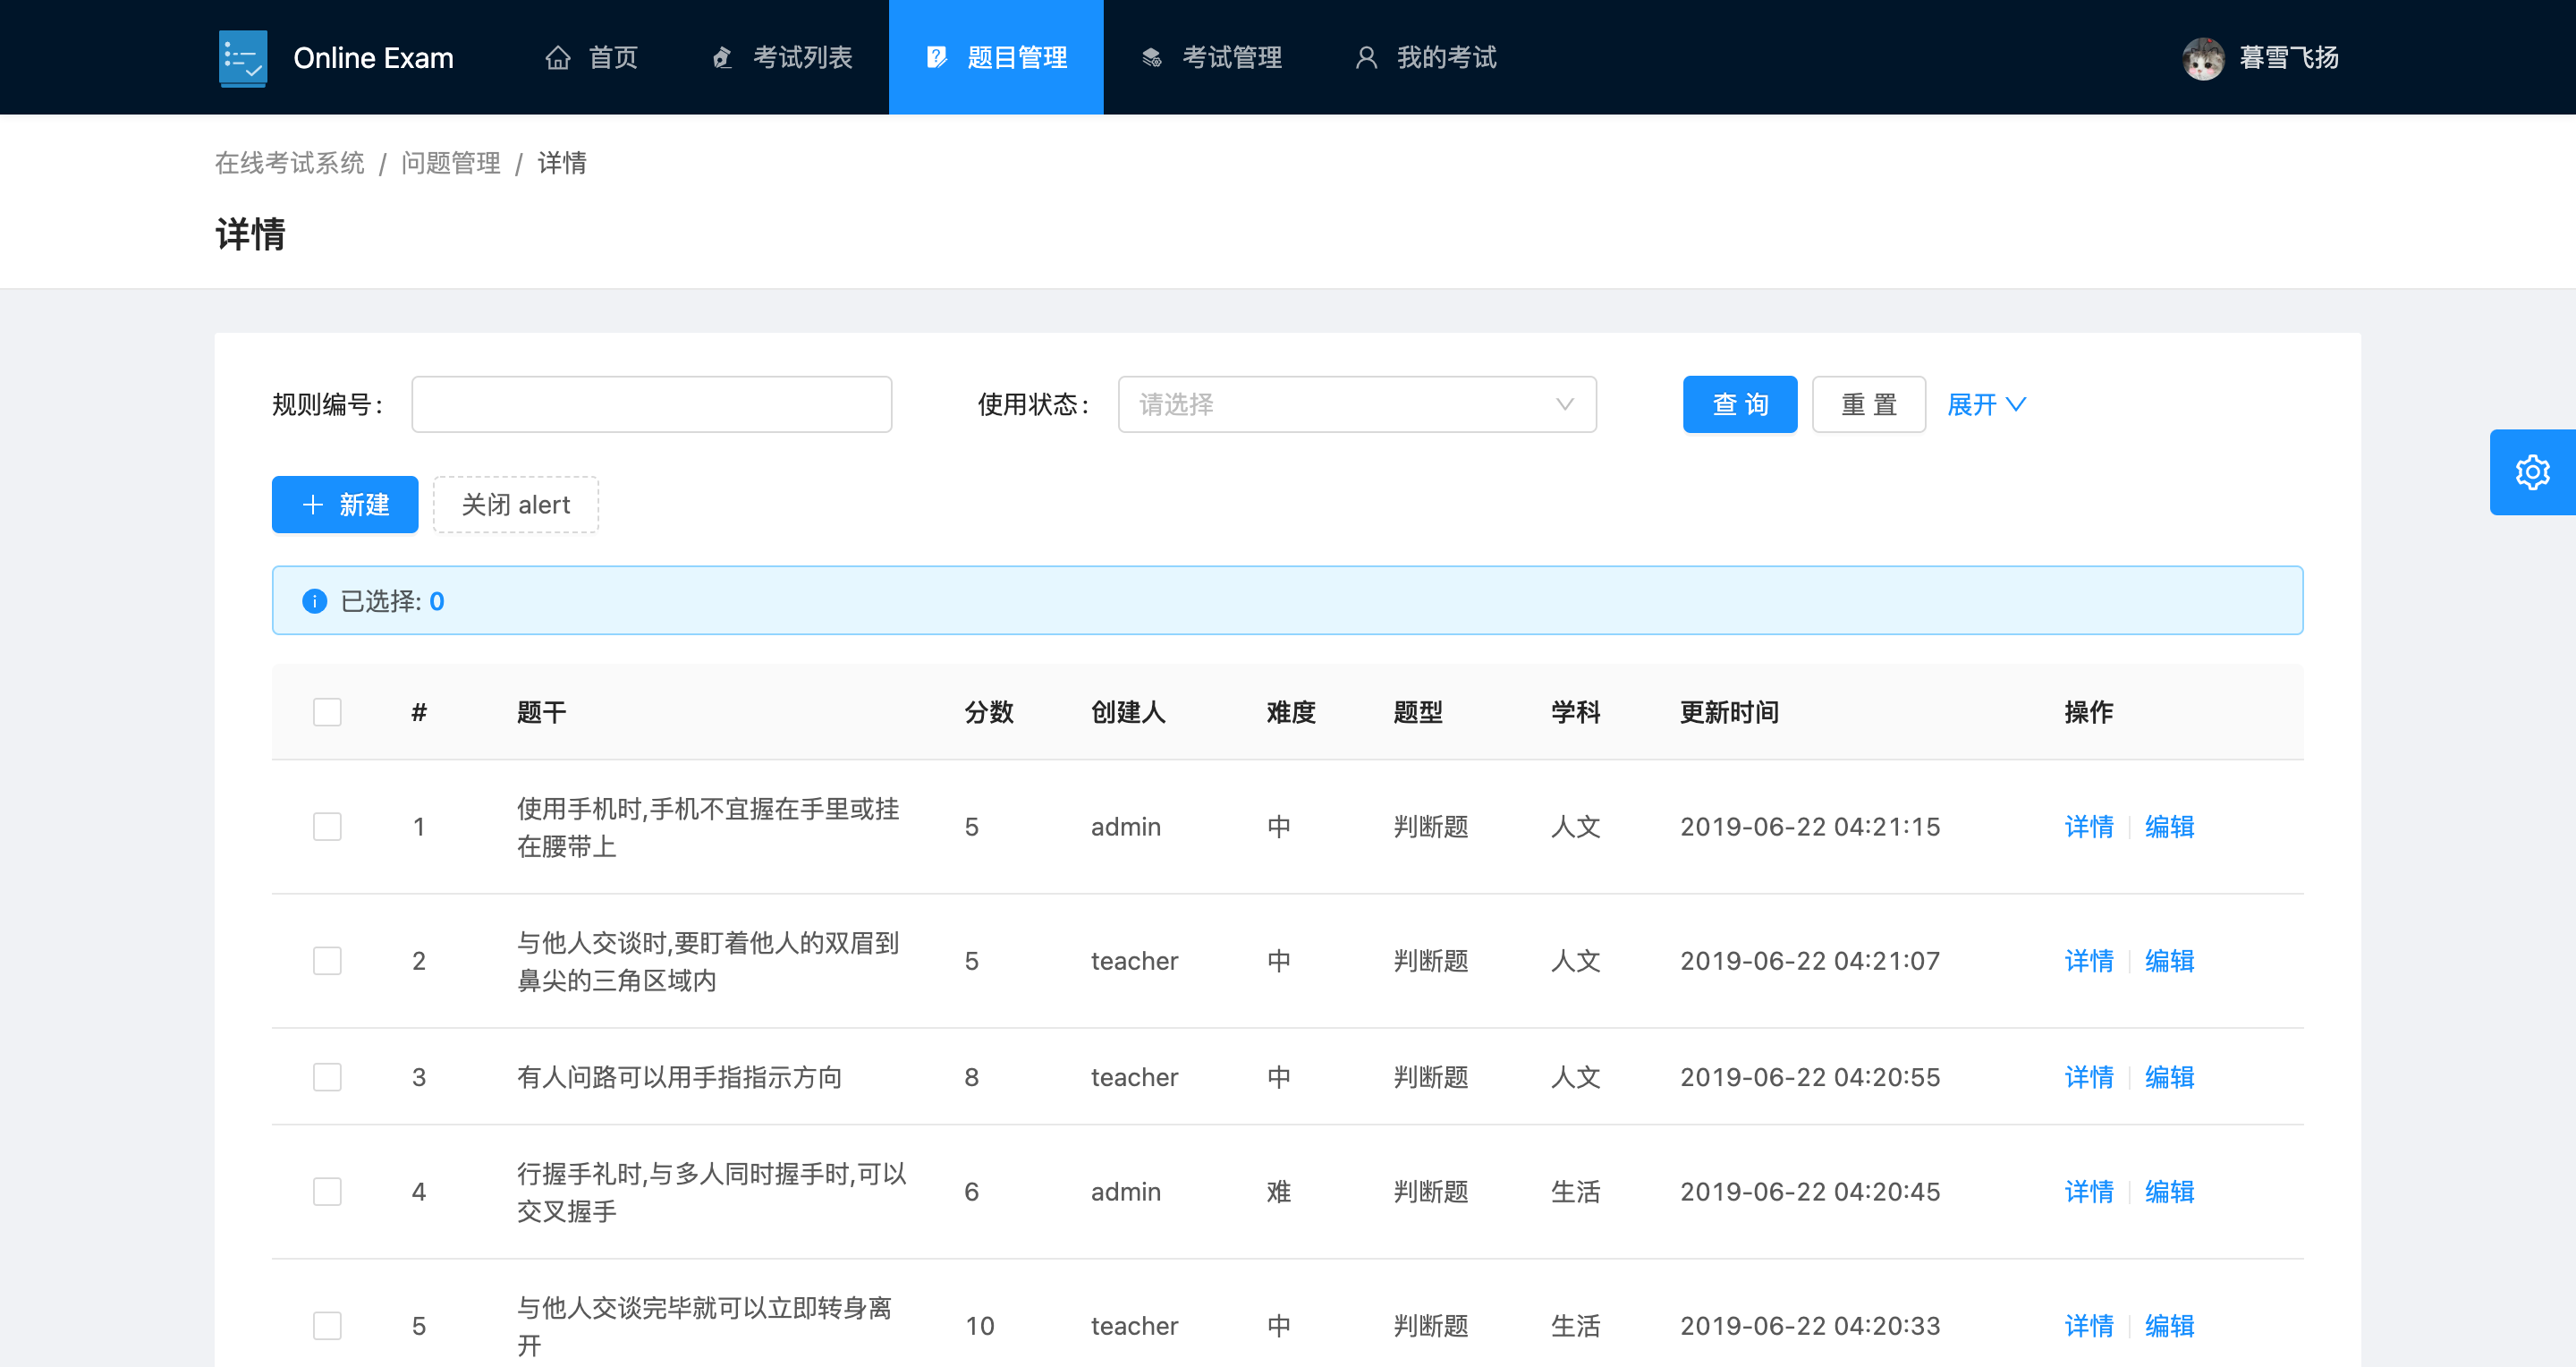
\includegraphics[width=\linewidth]{_images/题库模块截图.jpeg}
    \caption{题库模块}
\end{figure}
进入题库模块前需要先检查是否有进入的权限,如果没有则需要一定的 403 反馈。正常操作流程下,没有权限是无法通过点击事件进入题库,但也可能通过浏览器的地址栏 URL,通过路由器强行渲染出对应的题库 \lstinline!View! 组件,因此仍是需要在进入模块前进行权限检查。

如果有权限进入,则展示所有的题目,并可以进行分页操作、选择题库查看、选择具体题目操作。

分页操作,则需要在组件中托管具体的 \lstinline!current!、\lstinline!pageSize!、\lstinline!total! 数据,并注入 ant-d-v 提供的 \lstinline!<Pagination>!。分页请求时,向后端发起 \lstinline!/exam/question/list! 的 \lstinline!GET! 请求,并将 \lstinline!current! 和 \lstinline!pageSize! 作为参数。在后端 Controller 中接收请求,做处理。

\begin{lstlisting}[language=Java]
@GetMapping("/question/list")
@ApiOperation("获取问题的列表")
ResultVO<QuestionPageVo> getQuestionList(
    @RequestParam("pageNo") Integer pageNo, 
    @RequestParam("pageSize") Integer pageSize
) {
    ResultVO<QuestionPageVo> resultVO;
    
    try {
        QuestionPageVo questionPageVo = examService.getQuestionList(pageNo, pageSize);
        resultVO = new ResultVO<>(0, "获取问题列表成功", questionPageVo);
    } catch (Exception e) {
        e.printStackTrace();
        resultVO = new ResultVO<>(-1, "获取问题列表失败", null);
    }
    
    return resultVO;
}
\end{lstlisting}

选择具体题库,则展示具体题库下的题目。也可以进行修改题库信息、删除题库或新增题库。\upcite{ref12,ref14}

修改题库信息,可以修改题库的名称,或新增、删除其中包含的题目。

删除题库的操作,会将所有当前题库下的题目,与之解除关联。在具体的题库-题目 mapper 表中删除对应的映射。而不会删除具体的题目,即使已经没有任何题库与这些题目关联。但是这些题目仍是会在题库添加的时候,可选展示待加入。

新增题库的操作则会要求填写题库的基本信息,而后可以选择需要添加入题库的题目。也可以在创建成功以后,再通过修改题库的功能,对题库的题目做管理。

对于具体题目的操作,可以查看题目的详情,也可以对题目配置的属性做修改调整。

\begin{lstlisting}[language=Java]
@PostMapping("/question/update")
@ApiOperation("更新问题")
ResultVO<String> questionUpdate(@RequestBody QuestionVo questionVo) {
    // 完成问题的更新
    System.out.println(questionVo);
    try {
        examService.updateQuestion(questionVo);
        return new ResultVO<>(0, "更新问题成功", null);
    } catch (Exception e) {
        e.printStackTrace();
        return new ResultVO<>(-1, "更新问题失败", null);
    }
}
\end{lstlisting}

\begin{figure}[htb]
    \centering
    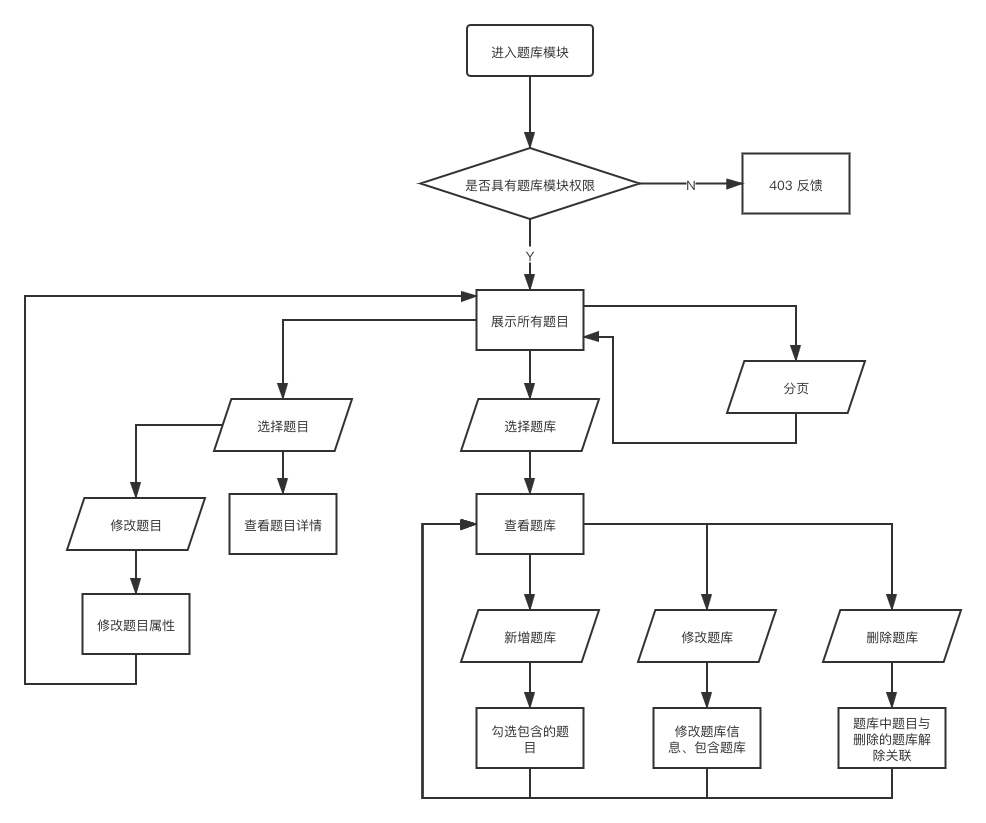
\includegraphics[width=\linewidth]{_images/题库模块.png}
    \caption{题库模块}
\end{figure}


\subsection{考卷模块}
进入考卷模块前需要先检查是否有进入的权限,如果没有则需要一定的 403 反馈。正常操作流程下,没有权限是无法通过点击事件进入考卷模块,但也可能通过浏览器的地址栏 URL,通过路由器强行渲染出对应的题库 \lstinline!View! 组件,因此仍是需要在进入考卷模块前进行权限检查。

\begin{lstlisting}[language=JavaScript]
export default {
  ... ...
  computed: {
      ... ...
      storeUserInfo: function(){
          return TokenManager.getToken().userInfo
      },
      ... ...
  },
  methods: {
      queryExamPaper: function(pageIndex){
          ... ...
          const userId = this.storeUserInfo?.id
          ... ...
          Requester.post(...)
          ... ...
      }
  },
  ... ...
}
\end{lstlisting}
如果有权限进入考卷模块,则需要从 store 中获取当前用户的 \lstinline!id!,并传入后端,并携带分页所需要的 \lstinline!current!、\lstinline!pageSize! 等信息。

在页面内可以进行创建考卷的操作。首先需要填写一些考卷的基本信息,例如考卷名称等。然后,需要去选择是否从题库中自动生成考卷的题目。如果选择从题库中自动生成,需要选择对应的题库,并且配置需要多少的客观题,及其中具体的题型和分值。如果需要手动选择添加的题目,则会展示系统中已有的题目,供手动选择。配置好考卷的基础信息以及具体的题目或选择的题库后,则向后端发起创建考卷的请求。生成考卷成功后,返回展示当前用户创建的考卷列表。

修改考卷的操作,可以修改考卷的基本信息,也可通过勾选框批量删除考题。或是通过弹窗查看未添加的考题,批量勾选添加。

删除考卷的操作,仅仅只删除考卷在数据库表中的记录,与考卷相关联的题目并不会被删除,即便是已经不归属与任何的考卷。
\begin{figure}[htb]
    \centering
    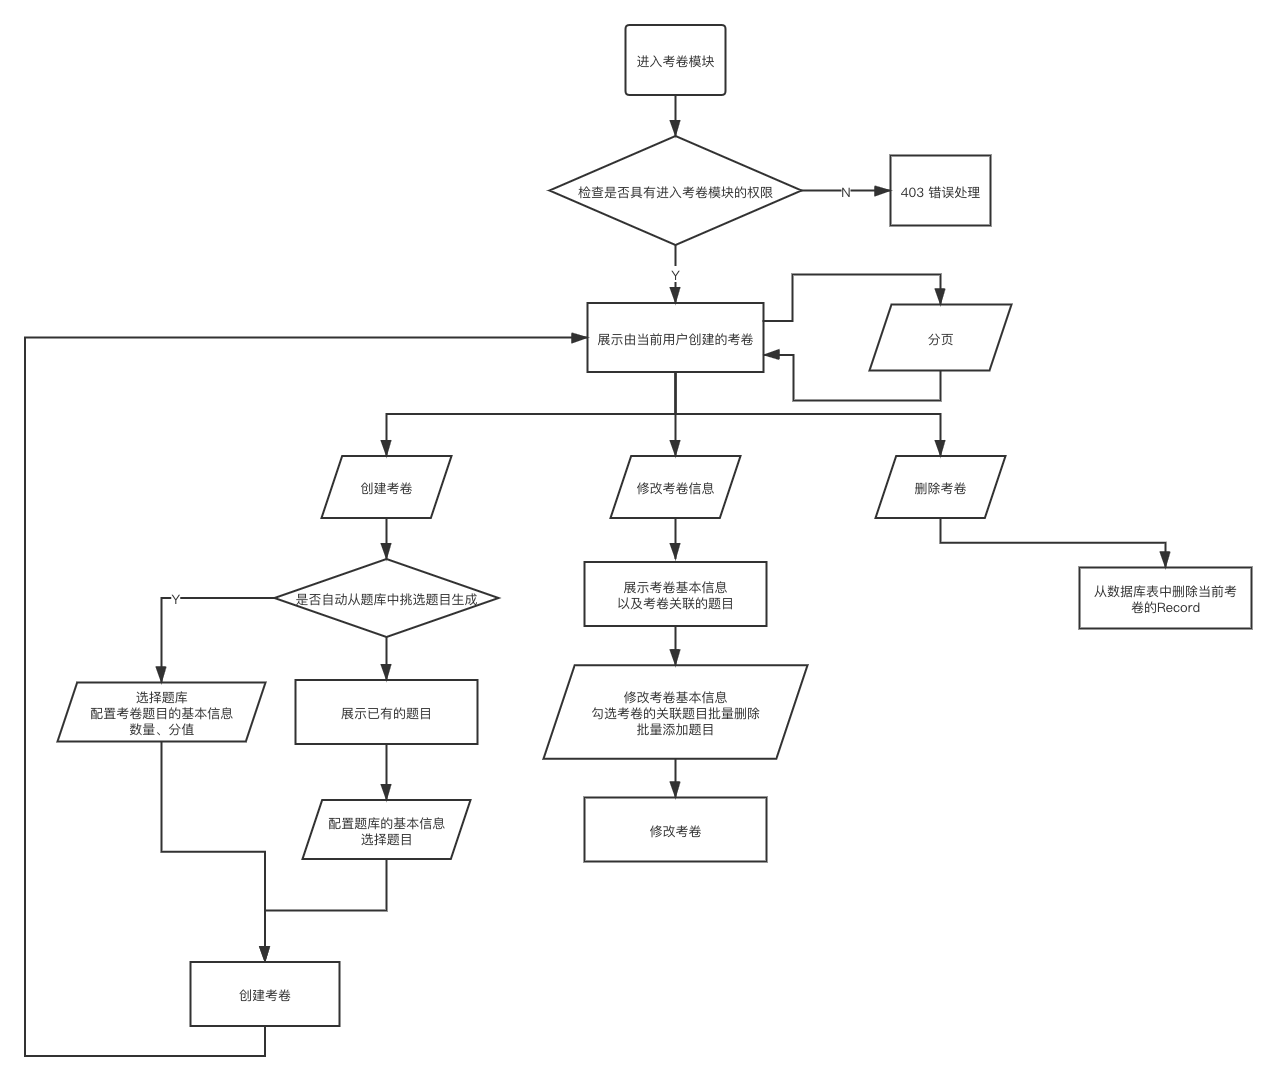
\includegraphics[width=\linewidth]{_images/考卷模块.png}
    \caption{考卷模块}
\end{figure}


\subsection{用户管理模块}
渲染用户模块前需要先检查是否有进入的权限,如果没有则需要一定的 403 反馈。正常操作流程下,没有权限是无法通过点击事件进入用户模块,但也可能通过浏览器的地址栏 URL,通过路由器强行渲染出对应的题库 View 组件,因此仍是需要在进入用户模块前进行权限检查。

进入用户模块后,以列表形式展示所有的用户。并可以通过 Select 框选择,按照不同的用户角色进行条件筛选,展示对应用户的情况。并且支持分页能力。

新增用户时需要填写用户的基本信息,并且需要选择用户的角色,赋予其权限划分。用户是通过 username 来区分的,所以在注册用户时,需要先判断 username 是否已存在,如果存在,则返回“用户名已存在”。如果不存在,将新用户信息添加到数据库。

修改用户和新增用户类似,也需要判断新的 username 是否已存在,如果不存在,则将修改后的信息更新到数据库。

删除用户仅仅将用户从 user 表中删除,而不删除所有相关联的其余表中的 creatorId(或将其设置为 -1)。这样就能保证其他原先创建的考卷、题库、题目,不会受到其创建人的用户被删除,而出现异常情况。其 creatorId 的失效也仅仅影响了查询部分。\upcite{ref7,ref22,ref17}

\begin{figure}[htb]
    \centering
    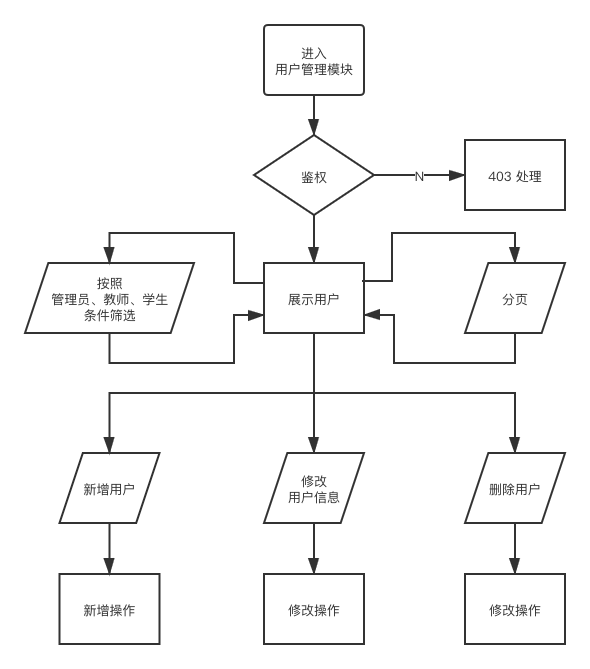
\includegraphics[width=0.7\linewidth]{_images/用户管理模块.png}
    \caption{用户管理模块}
\end{figure}


\subsection{考试模块}
所有的用户都有权限进入考试模块。首先展示的是所有的考试,所以在进入页面前会先请求所有的考试信息。
\begin{lstlisting}[language=JavaScript]
function getExamCardList() {
  return axios({
    url: api.ExamCardList,
    method: 'get',
    headers: {
      'Content-Type': 'application/json;charset=UTF-8'
    }
  })
}
\end{lstlisting}
\begin{lstlisting}[language=Java]
@GetMapping("/card/list")
@ApiOperation("获取考试列表,适配前端卡片列表")
ResultVO<List<ExamCardVo>> getExamCardList() {
    // 获取考试列表卡片
    ResultVO<List<ExamCardVo>> resultVO;
    try {
        List<ExamCardVo> examCardVoList = examService.getExamCardList();
        resultVO = new ResultVO<>(0, "获取考试列表卡片成功", examCardVoList);
    } catch (Exception e) {
        e.printStackTrace();
        resultVO = new ResultVO<>(-1, "获取考试列表卡片失败", null);
    }
    return resultVO;
}
\end{lstlisting}
其中,可以进行条件筛选。可以按照已结束的考试、参加过的考试、可参加的仍在有效时间内的、未开始的,进行对考试列表的筛选。如果是展示的参加过的考试,点击事件会展示考试的详情。包括考试的答案、问题的正确答案、正确答案的解析,以及考试的得分。

在考试列表中,可以选择考试参加。点击选择的考试将跳转到答题系统中,即可进行答题。答题过程中将会进行计时操作。提交答案前,将会进行检查是否有未作答的题目,如有则拒绝提交。提交考试后将跳转回考试模块的最初页面。

\begin{figure}[htb]
    \centering
    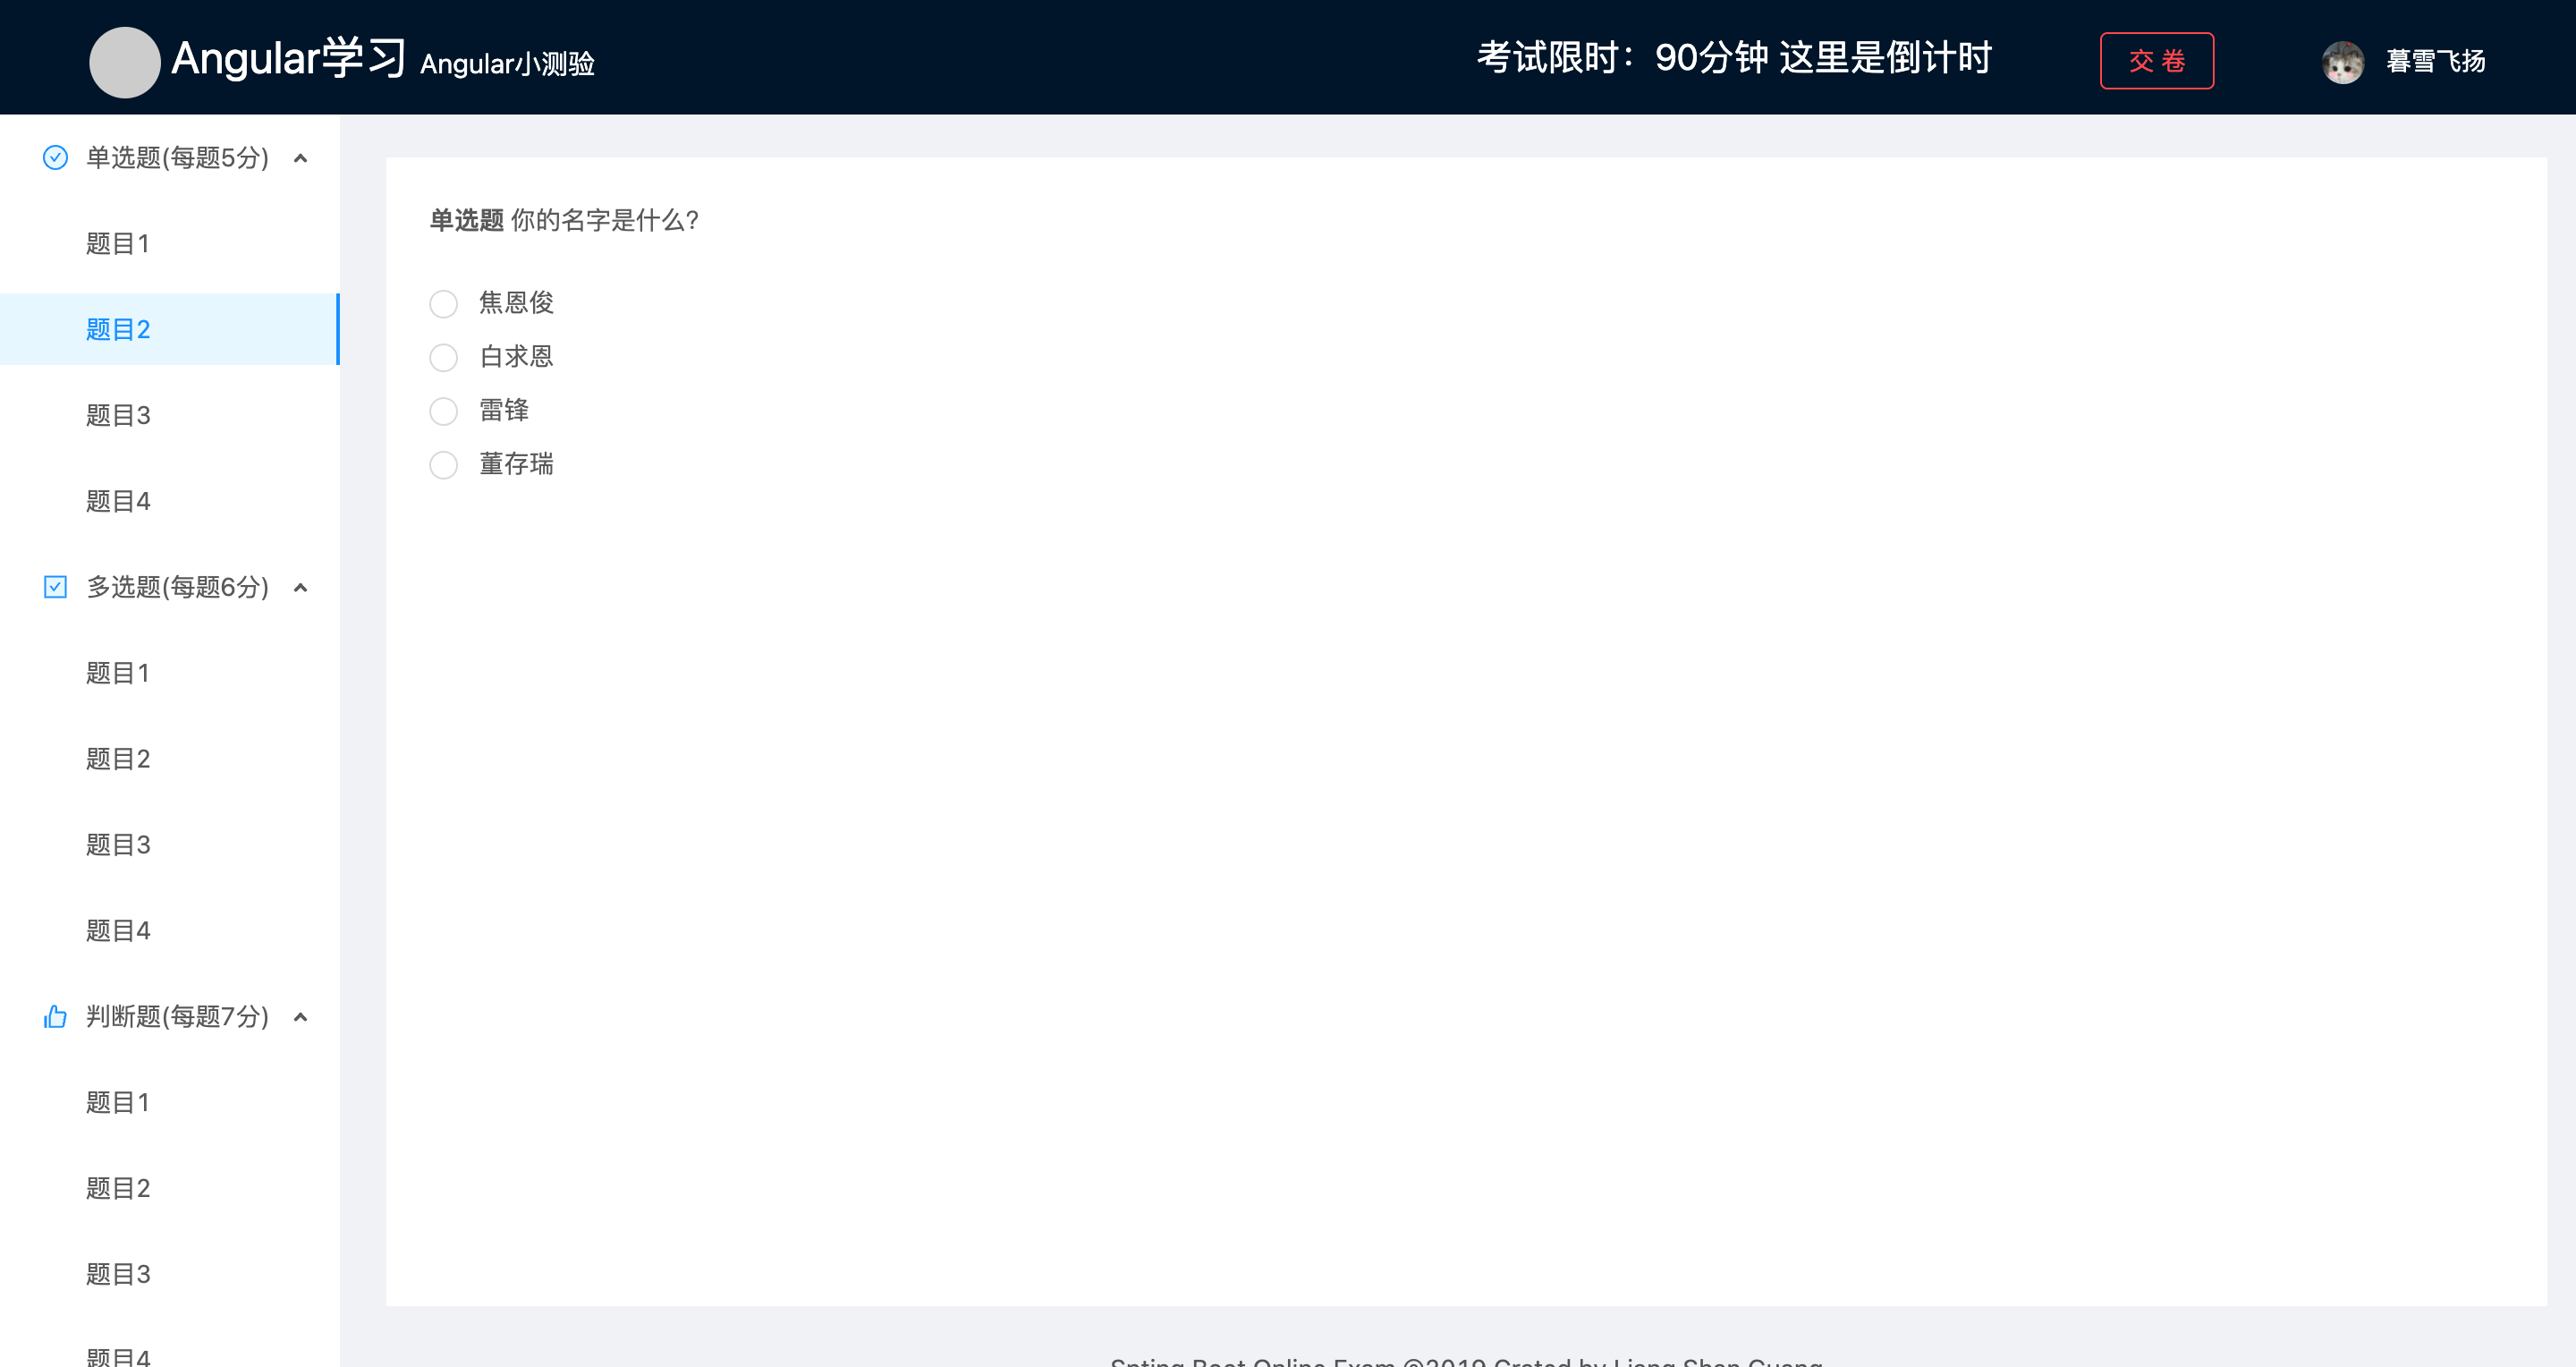
\includegraphics[width=\linewidth]{_images/答题系统.png}
    \caption{答题系统}
\end{figure}

创建考试并不是所有用户角色都拥有的权限。因而,创建考试的按钮需要根据当前登录的用户角色,通过 
\lstinline!v-if! 的方式决定是否渲染。点击创建考试,需要选择考试使用的考卷,以及填写考试的基本信息、起始时间、结束时间,以及时间限制。\upcite{ref18}

\begin{figure}[ht!]
    \centering
    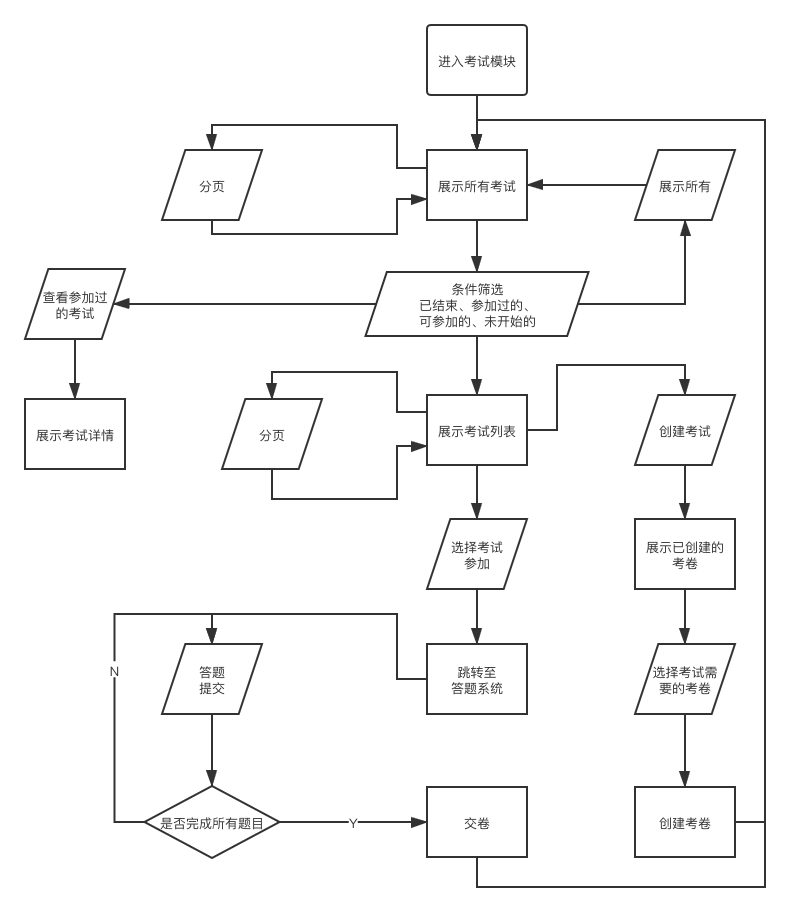
\includegraphics[width=\linewidth]{_images/考试模块.png}
    \caption{考试模块}
\end{figure}


\subsection{章节小结}
本章主要是针对系统设计章节,划分出的系统的四个核心功能模块:题库、考卷、用户、考试模块,进行了针对性的实现层面的阐述。其中着重通过业务逻辑的伪代码,用户操作的流程图等形式,配以相应的文字说明,来阐明项目中对于这几个核心模块的实现情况。
\section{系统测试}
\section{总结与展望}

% \addcontentsline{toc}{section}{参考文献}
% \bibliography{bibfile}
\section*{参考文献}
\addcontentsline{toc}{section}{参考文献}

\begingroup
% 隐藏自带的title
\def\section*#1{}

\begin{thebibliography}{99}

\bibitem{ref0}Nakamoto S . Bitcoin: A Peer-to-Peer Electronic Cash System[J]. consulted.
\bibitem{ref1}杨骏佶. 面向计算机硬件的远程虚拟实验服务[D]. 江苏大学, 2019.
\bibitem{ref2}魏婙. 社区管理系统的设计与实现[D]. 哈尔滨工业大学, 2016.
\bibitem{ref3}杨胜超~张瑞军. 基于二分图最优匹配算法的毕业论文选题系统[D]. 计算机系统应用, 2008.
\bibitem{ref4}杨晓. 云师大课程考试系统的设计与实现[D]. 电子科技大学, 2013.
\bibitem{ref5}严俊杰. 基于Spring Cloud的回顾式阅读辅助系统的设计与实现[D]. 南京大学, 2019.
\bibitem{ref6}孙阳. 南师大泰州学院教学评估管理信息系统的设计与实现[D]. 电子科技大学, 2014.
\bibitem{ref7}高淼. 电路板故障诊断系统TPS运行及数据管理模块设计与实现[D]. 电子科技大学, 2011.
\bibitem{ref8}李炎平. 一个物料编码与清单生成器系统的设计与实现[D]. 华中科技大学, 2015.
\bibitem{ref9}郭昕. 高校毕业生跟踪反馈系统的设计与实现[D]. 天津大学, 2015.
\bibitem{ref10}李建忠~胡新刚~孟志强. 运用虚拟化、云计算搭建集团企业云[D]. 创新世界周刊, 2019.
\bibitem{ref11}佘春华. 基于认知灵活性理论的高中物理虚拟实验教学平台的设计与开发[D]. 广西师范学院, 2011.
\bibitem{ref12}姚迪. 河南电力公司网络培训考试系统的设计与应用[D]. 华北电力大学, 2017.
\bibitem{ref13}肖敏 郭秋萍 莫祖英. 政府数据开放发展历程及平台建设的差异分析——基于四个国家的调[D]. 图书馆理论与实践, 2019.
\bibitem{ref14}徐英. 基于java的数学自测评估系统的设计与实现[D]. 电子科技大学, 2013.
\bibitem{ref15}Drijvers M, Gorbunov S, Neven G, et al. Pixel: Multi-signatures for consensus[C]//29th {USENIX} Security Symposium ({USENIX} Security 20). 2020: 2093-2110.
\bibitem{ref16}赵世平. 网络数据流监控管理平台的设计与实现[D]. 电子科技大学, 2012.
\bibitem{ref17}夏婷婷. 基于FPGA的嵌入式环境监测系统设计[D]. 西北大学, 2015.
\bibitem{ref18}周高嵚. 基于白箱测试的源代码在线评测系统[D]. 北京化工大学, 2005.
\bibitem{ref19}林潇. 移动web端网站无障碍人工检测系统的设计与实现[D]. 浙江大学, 2018.
\bibitem{ref20}王立波. 基于Web Service的掌上酒店预订系统的设计与实现[D]. 电子科技大学, 2014.
\bibitem{ref21}林洁璇. 信息技术网络考试系统的研究与设计[D]. 韩山师范学院潮州师范分院, 2013.
\bibitem{ref22}黄庆庆. 兰州大学新闻与传播学院网站创新发展方案[D]. 兰州大学, 2017.
\bibitem{ref23}Wang R, Ye K, Meng T, et al. Performance Evaluation on Blockchain Systems: A Case Study on Ethereum, Fabric, Sawtooth and Fisco-Bcos[C]//International Conference on Services Computing. Springer, Cham, 2020: 120-134.

\end{thebibliography}

\endgroup
\clearpage

% \clearpage

\section*{致谢}
\addcontentsline{toc}{section}{致谢}

\end{document}
